\documentclass[12pt,a4paper,titlepage,final]{article}
\usepackage[czech]{babel}
\usepackage[utf8]{inputenc}
\usepackage[bookmarksopen,colorlinks,plainpages=false,urlcolor=blue,unicode]{hyperref}
\usepackage{url}
\usepackage{float}
\usepackage{ifthen}
\usepackage[dvipdf]{graphicx}
\usepackage[top=3.5cm, left=2.5cm, text={17cm, 24cm}, ignorefoot]{geometry}

\begin{document}
\newpage

%%%%%%%%%%%%%%%%%%%%%%%%%%%%%%%%%%%%%%%%%%%%%%%%%%%%%%%%%%%%%%%%%%%%%%%%%%%%%%
% titulní strana
\def\name{Lukáš Vokráčko}
\def\login{xvokra00}
\def\subject{Paralelní a distribuované algoritmy}
\def\project{Minimum Extraction Sort}

\newboolean{frontpage}
% \setboolean{frontpage}{true}
\setboolean{frontpage}{false}

\ifthenelse{\boolean{frontpage}}
{
	\pagestyle{empty}
	\begin{titlepage}

% \vspace*{1cm}
\begin{figure}[!h]
\centering
% \includegraphics[width=3.5cm,keepaspectratio]{fit-logo.eps}
\includegraphics[width=7cm,keepaspectratio]{logo.eps}

\end{figure}

\vfill

\begin{center}
\begin{Huge}
	\subject
\end{Huge}
\\
\begin{Large}
	\project
\end{Large}
\end{center}

\vfill

\begin{center}
\begin{Large}
\today
\end{Large}
\end{center}

\vfill

\begin{flushleft}
\begin{large}
\begin{tabular}{ll}
Autor: & \name, \url{\login@stud.fit.vutbr.cz} \\
 & Fakulta Informačních Technologií \\
 & Vysoké Učení Technické v~Brně \\
\end{tabular}
\end{large}
\end{flushleft}
\end{titlepage}

	\tableofcontents
	\newpage
	\pagestyle{plain}
}
{
	\pagestyle{plain}
	% \vspace*{2px}
	\hfill \name, \login \\
	\vspace*{5px}
	{\LARGE \subject}  \\
	{\LARGE \project}  \\
}

\pagenumbering{arabic}
\setcounter{page}{1}
%%%%%%%%%%%%%%%%%%%%%%%%%%%%%%%%%%%%%%%%%%%%%%%%%%%%%%%%%%%%%%%%%%%%%%%%%%%%%%

\section{Analýza algoritmu}
Algoritmus \texttt{Minimum extraction sort} využívá k řazení stromové struktury, z čehož vyplývá, že pro $n$ prvků bude mít strom 
$log(n) + 1$ úrovní. Jelikož všechny prvky začínají svou cestu stromem v listovém uzlu, musí každý prvek projít $log(n)$ úrovněmi, než se dostane do kořenu.
Kořen potřebuje dva kroky pro zpracování každého prvku, tudíž výsledná časová složitost $t(n)$ je $2n$ pro každý prvek kromě prvního a $log(n)$ pro první prvek.
Výsledná časová složitost tedy bude $t(n) = 2*n - 1 + log(n)$. Prostorová složitost $p(n)$ je  rovna počtu potřebných procesorů, který činí $2*n - 1$, neboť každý prvek vyžaduje samostatný procesor plus $n-1$ procesorů pro každý nelistový uzel stromu. Celková cena je pak vypočtena jako $c(n) = t(n) * p(n)$.\\
$t(n) = 2*n-1+log(n) = O(n)$ \\
$p(n) = 2*n-1 = O(n)$ \\
$c(n) = O(n)*O(n)= O(n^2) $.

\section{Implementace}
Program je implementován v jazyce C s využití knihovny \url{https://www.open-mpi.org/}.
Pro spuštění je vytvořen skript \texttt{test}, který vygeneruje soubor \texttt{numbers} s náhodnými čísly,
přeloží program \texttt{mes} a spustí ho v prostředí \texttt{MPI}. Výstupem programu je vypsaná neseřazená posloupnost čísel na prvním řádku.
Na další řádcích následuje již seřazená posloupnost a to od nejmenšího prvku.

\section{Experimenty}
Program byl testován pro počet prvků odpovídajícím $2^n$ pro $n = 1 .. 6$. Pro větší množství prvků se již nepodařilo spustit odpovídající počet procesorů.
Počty prvků, který by neodpovídal mocninám dvou testován nebyl, neboť algoritmus \texttt{Minimum extraction sort} pro $(2^n,2^{n+1})$ prvků díky své stromové struktuře vždy
vyžaduje $2^{n+2}-1$ procesorů a tudíž by se výsledné hodnoty shodovaly s naměřenými hodnotami pro $2^{n+1}$ prvků.

Testování probíhalo na stroji s jedním procesorem, tudíž MPI simulovalo procesory procesy. Z toho
vyplývá i naměřená časová složitost $O (n^2)$, která odpovídá celkové ceně algoritmu $c(n) = p(n)*t(n) = O (n) * O (n)$,
neboť na jednoprocesorovém systému nepoběží úlohy paralelně. V následujícím grafu jsou zaneseny hodnoty naměřené pro řazení $2^n, n = {1,2,..,6}$ hodnot.
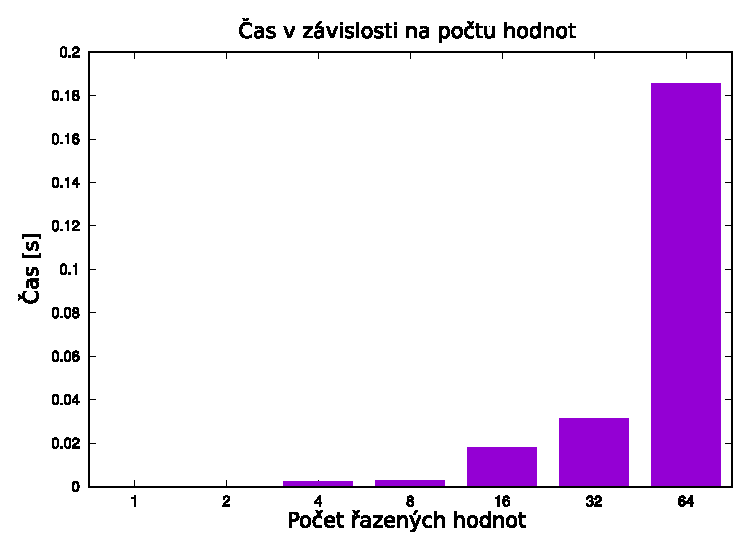
\includegraphics[width=14cm,keepaspectratio]{time.eps}

\section{Komunikační protokol}
Každý uzel vyjma kořene odesílá a přijímá svoji hodnotu od přímého rodičovského uzlu.
Pro nelistové uzly dochází po přijetí hodnot obou synů k porovnání jejich hodnot a 
uzlu, jež poslal menší hodnotu je odeslána zpět hodnota reprezentující prázdný uzel zatímco druhému uzlu
je odeslána zpět jeho původní hodnota. \\
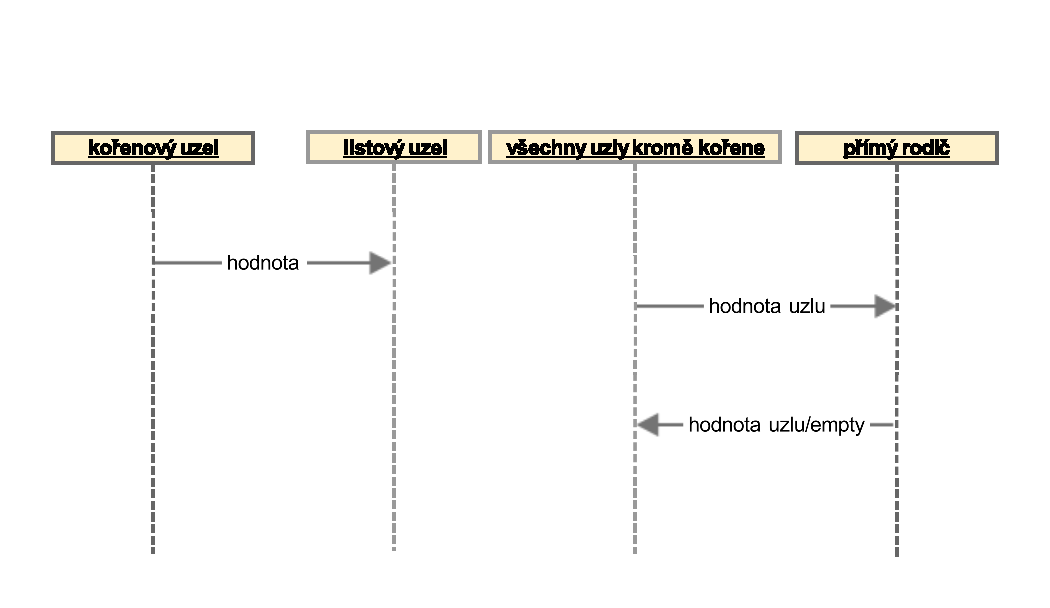
\includegraphics[width=14cm,keepaspectratio]{sequence.eps}

\section{Závěr}
Naměřené hodnoty při experimentování neodpovídají časové složitosti $t(n) = O(n)$, neboť byly prováděny na jednoprocesorovém stroji a tudíž by naměřené hodnoty měly 
odpovídat celkové ceně algoritmu $c(t) = O(n^2)$, neboť všechny kroky všech procesorů jsou vykonávány sekvenčně, čemuž také odpovídají naměřené výsledky.

\end{document}
